
\documentclass[11pt, titlepage, oneside, a4paper]{article}
\usepackage[T1]{fontenc}
\usepackage{hyperref}
\usepackage[utf8]{inputenc}
\usepackage[english]{babel}
\usepackage{amssymb, graphicx, fancyhdr}
\usepackage{listings}
\lstset{breaklines=true} 
\lstset{numbers=left, numberstyle=\scriptsize\ttfamily, numbersep=10pt, captionpos=b} 
\lstset{basicstyle=\small\ttfamily}
\newcommand{\inlineCode}{\lstinline[basicstyle=\normalsize\ttfamily]}
\addtolength{\textheight}{20mm}
\addtolength{\voffset}{-5mm}
\renewcommand{\sectionmark}[1]{\markleft{#1}}

% \Section ger mindre spillutrymme, använd dem om du vill
\newcommand{\Section}[1]{\section{#1}\vspace{-8pt}}
\newcommand{\Subsection}[1]{\vspace{-4pt}\subsection{#1}\vspace{-8pt}}
\newcommand{\Subsubsection}[1]{\vspace{-4pt}\subsubsection{#1}\vspace{-8pt}}
	
% appendices, \appitem och \appsubitem är för bilagor
\newcounter{appendixpage}

\newenvironment{appendices}{
	\setcounter{appendixpage}{\arabic{page}}
	\stepcounter{appendixpage}
}

\newcommand{\appitem}[2]{
	\stepcounter{section}
	\addtocontents{toc}{\protect\contentsline{section}{\numberline{\Alph{section}}#1}{\arabic{appendixpage}}}
	\addtocounter{appendixpage}{#2}
}

\newcommand{\appsubitem}[2]{
	\stepcounter{subsection}
	\addtocontents{toc}{\protect\contentsline{subsection}{\numberline{\Alph{section}.\arabic{subsection}}#1}{\arabic{appendixpage}}}
	\addtocounter{appendixpage}{#2}
}

% Ändra de rader som behöver ändras
\def\inst{Tillämpad fysik och elektronik}
\def\typeofdoc{Laborationsrapport}
\def\course{Script och webbrogrammering 7,5 hp}
\def\pretitle{Laboration 5}
\def\title{PHP och Databaser}
\def\name{Christer Jakobsson}
\def\username{dv12cjn}
\def\email{\username{}@cs.umu.se}
\def\graders{Ola Ågren, Kalle Prorok}



% Här brjar själva dokumentet
\begin{document}

	% Skapar framsidan (om den inte duger: gör helt enkelt en egen)
	\begin{titlepage}
		\thispagestyle{empty}
		\begin{large}
			\begin{tabular}{@{}p{\textwidth}@{}}
				\textbf{UMEÅ UNIVERSITET \hfill \today} \\
				\textbf{Institutionen för \inst} \\
				\textbf{\typeofdoc} \\
			\end{tabular}
		\end{large}
		\vspace{10mm}
		\begin{center}
			\LARGE{\pretitle} \\
			\huge{\textbf{\course}}\\
			\vspace{10mm}
			\LARGE{\title} \\
			\vspace{15mm}
			\begin{large}
				\begin{tabular}{ll}
					\textbf{Namn} & \name \\
					\textbf{E-mail} & \texttt{\email} \\
					\textbf{Adress} & \url{http://shinowa.tk}
				\end{tabular}
			\end{large}
			\vfill
			\large{\textbf{Handledare}}\\
			\mbox{\large{\graders}}
		\end{center}
	\end{titlepage}


	% Fixar sidfot
	\lfoot{\footnotesize{\name, \email}}
	\rfoot{\footnotesize{\today}}
	\lhead{\sc\footnotesize\title}
	\rhead{\nouppercase{\sc\footnotesize\leftmark}}
	\pagestyle{fancy}
	\renewcommand{\headrulewidth}{0.2pt}
	\renewcommand{\footrulewidth}{0.2pt}

	
	
	\pagenumbering{arabic}
	% I Sverige har vi normalt inget indrag vid nytt 
	\setlength{\parindent}{0pt}
	% men däremot lite mellanrum
	\setlength{\parskip}{10pt}

	% Lägger in rubrik (finns \section, men då får man mycket spillutrymme)
	
	\Section{Del 1}
		\Subsection{Problembeskrivning}
		Tanken med denna del av uppgiften är att skriva ett php script som hanterar något som skrivits in i ett formulär, jag ska således skapa en html sida med ett 
		formulär som, när användaren trycker på \emph{Submit} ska hanteras av ett php script som jag också ska skapa. 
		Scriptet ska även hantera standardinformation som tex IP-nummer och tid.
		
		\Subsection{Användarhandledning}
		Denna del går att komma åt via:\\ \url{http://shinowa.tk/lab5/formWithStandardInfo.html}.
		Eller genom att först använda länken \url{shinowa.tk} och sedan klicka under Del 1 \emph{Fristående php: Add Form}.
		
		När man har navigerat till sidan så får man fylla i alla fält:
		\begin{itemize}
		 \item[First Name:] Krävs, får bara innehålla stora och små bokstäver samt tecknet \emph{-}.
		 \item[Last Name:] Krävs, får bara innehålla stora och små bokstäver samt tecknet \emph{-}.
		 \item[E-mail:] Måste innehålla @ (snabel a)
		 \item[Password:] Krävs, måste vara samma som \emph{Retype Password}
		 \item[Retype Password:] Krävs, måste vara samma som \emph{Password}
		 \item[Telephone:] Krävs, måste vara ett nummer.
		 \item[Sex:] Krävs.
		 \item[Favorite Color:] Krävs.
		\end{itemize}
		
		Om användaren vill börja om med att skriva formuläret så kan denne trycka på \emph{Reset} för att nollställa alla fält.
		När formuläret är ifyllt så trycker man på \emph{Submit} och kommer då att komma till en sida som innehåller php kod för att hantera datat ifrån formuläret.
		
		Först så valideras varje fält enligt reglerna i listan ovan och om alla fält är korrekt ifyllda så visas värdena på sidan tillsammans med standardinformation såsom ip-nummer, webbläsare samt datum och tid.
		\newpage
		\Subsection{Exempelkörningar}
		
		  \Subsubsection{Korrekt ifyllt formulär}
		  Jag skriver in korrekta värden i varje fält och trycker på \emph{Submit}.
		  \begin{figure}[h]
		  \centering
		  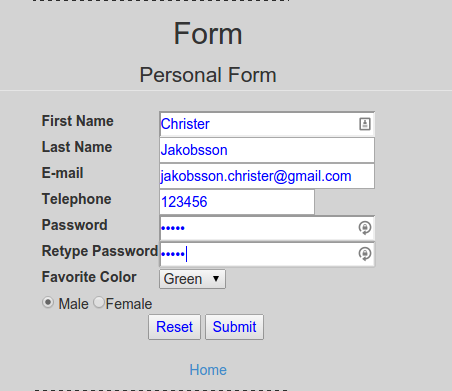
\includegraphics[width=90mm]{del1_formfilled.png}
		  \caption{Formulär med korrekt ifyllda fält}
		  \end{figure}

		  Jag ser resultatet av det jag skrivit in i formuläret. Notera att lösenorden är identiska.
		  \begin{figure}[ht!]
		  \centering
		  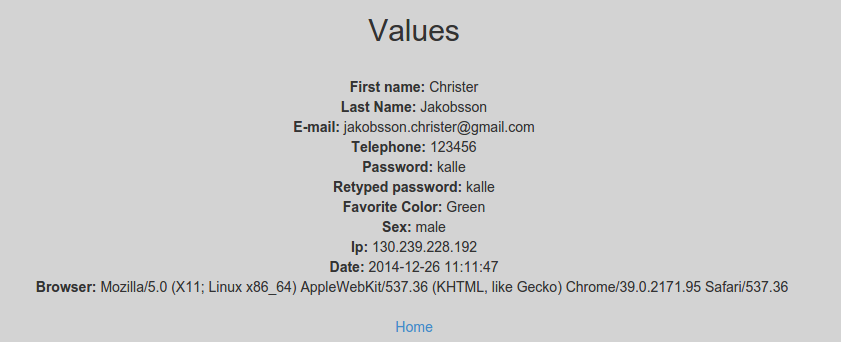
\includegraphics[width=120mm]{del1_result.png}
		  \caption{Resultat efter \emph{Submit}}
		  \end{figure}
		  
		  Kommentar: Fungerar som tänkt, i en riktig version skulle man inte hantera ett lösenord så här men detta är bara till för att jag vill prova password typen i formuläret.
		\newpage
		\Subsubsection{Felaktigt \emph{First Name}}
		Jag skriver in ett namn med siffror, vilket inte ska godkännas och trycker på \emph{Submit}.
		\begin{figure}[ht!]
		\centering
		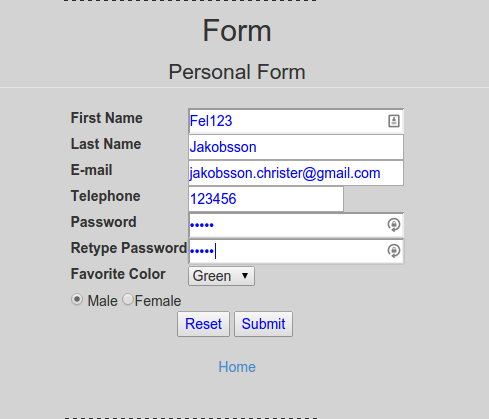
\includegraphics[width=90mm]{del1_first_name_fel.png}
		\caption{Felaktigt First Name}
		\end{figure}

		Jag ser att detta inte godkändes och at felet var i \emph{First Name}
		\begin{figure}[ht!]
		\centering
		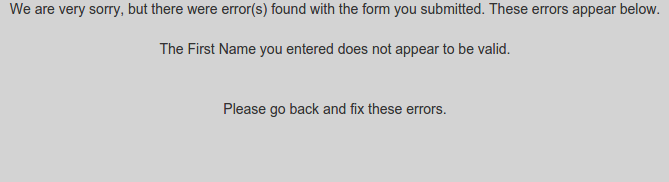
\includegraphics[width=120mm]{del1_first_name_fel_result.png}
		\caption{Resultat efter \emph{Submit}}
		\end{figure}
		
		\newpage
		\Subsubsection{Två felaktiga fält}
		Jag skriver in ett förnamn och ett efternamn med siffror, vilket inte ska godkännas, resterande fält är korrekta.\\ 
		\emph{First Name}: test123 \\
		\emph{Last Name}: test123 \\
		Trycker på \emph{Submit}.
				\begin{figure}[ht!]
				\centering
				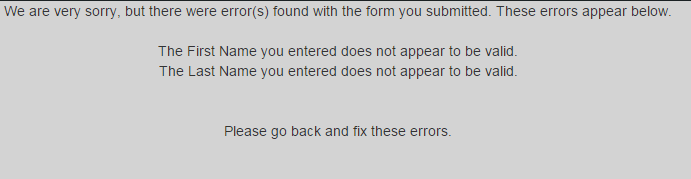
\includegraphics[width=90mm]{del1_tvafel.png}
				\caption{Felaktigt First Name}
				\end{figure}
		
			Kommentar: Här kan vi se att användaren får information om vilka fält som är fel, trots att det är mer än ett fält som är fel.
				
				\Subsubsection{Felaktigt \emph{E-mail}}
				Jag skriver in en felaktig E-mail, utan @.
				\begin{figure}[ht!]
				\centering
				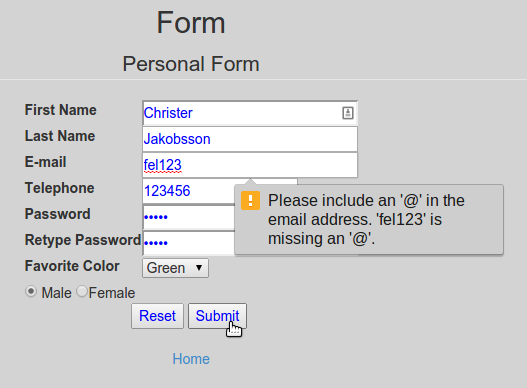
\includegraphics[width=90mm]{del1_fel_email.png}
				\caption{Vy vid klick av submit}
				\end{figure}
		
		\newpage
		\Subsubsection{Felaktigt telefonnummer}
		Jag skriver in ett nummer som innehåller bokstäver.
		
		\begin{figure}[ht!]
		\centering
		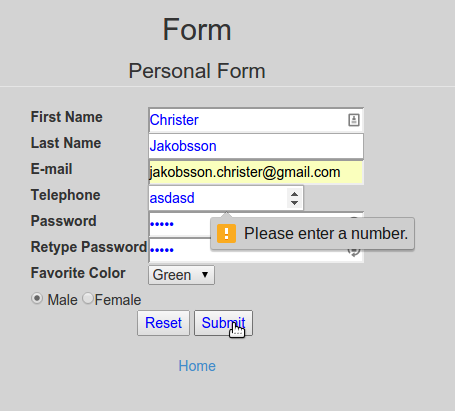
\includegraphics[width=90mm]{del1_fel_telefon.png}
		\caption{Vy vid klick av submit}
		\end{figure}
		
		\Subsubsection{Lösenord som inte matchar}
		Jag skriver in lösen1 i \emph{Password} och lösen2 i \emph{Retype Password} och klickar på \emph{Submit}
		\begin{figure}[ht!]
		\centering
		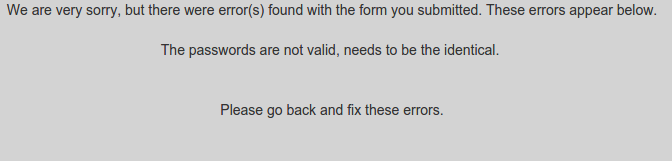
\includegraphics[width=90mm]{del1_fel_omatch.png}
		\caption{Vy efter Submit}
		\end{figure}

		\newpage
	\Section{Del 2}
		\Subsection{Problembeskrivning}
		Denna del av laborationen har gått ut på att göra ett eller flera skript som presenterar och ändrar något i en databas. Om man har tänkt att göra ett enkelt bokhanteringssystem i projektet så kan man göra skript som är en prototyp till det.
		Jag använder mig av html och php för att skapa några enkla sidor där användaren kan lägga till en bok, ta bort en bok, ändra en boks fält och en sida där man kan se alla böcker.
		
		\Subsection{Användarhandledning}
		Denna del innehåller flera små delar där alla hanterar bokhanteringsdatabas, delen innehåller tre stycken formulär som kan användas för att manipulera databasen.
		Dessa formulär finns på: \url{http://shinowa.tk} under rubriken, del 2.
		
		\Subsubsection{Lägga till bok}
		Detta formulär liknar hur det fungerade att lägga till en bok i det grafiska gränssnittet i laboration 4. Alla fält förutom \emph{Comments} måste vara ifyllda.
		\emph{Date Read} måste vara ett datum, och \emph{Grade} måste vara en siffra emellan 1-5.
		\emph{Genre} och \emph{Genre2} är listboxes med fördefinierade val, \emph{Genre2} ändrar dess värden beroende på vilket värde som är valt i \emph{Genre}.
		
		Användaren fyller i formuläret och klickar på \emph{Add book} för att lägga in det i databasen, i detta steg så valideras fälten och om alla fält är korrekta så läggs det in i databasen.
		Om något inte är korrekt ifyllt så visas en popup med vilket fält som måste korrigeras för att kunna lägga in bokdata't.
		

		Regler för fält:
		\begin{itemize}
		 \item[Author:] Krävs, får innehålla A-Z, a-z 
		 \item[Title:] Krävs, får innehålla alla tecken
		 \item[Date Read:] Krävs, måste vara i ett datum format.
		 \item[Genre:] Krävs, Listbox
		 \item[Genre2:] Krävs, Listbox
		 \item[Grade:] Krävs, Listbox
		 \item[Comments:] Valfri, kan innehålla alla tecken
		\end{itemize}
		
		Detta formulär finns på: \url{http://shinowa.tk/lab5/book_addForm.html}
		
		\Subsubsection{Ta bort bok}
		
		Detta formulär används för att ta bort en bok ifrån databasen, användaren får skriva in titeln på den bok som ska tas bort och sedan klicka på \emph{Remove Title}.
		Sedan så visas en resultatsida där man kan se om titeln har tagits bort, om ingen titel tagits bort så finns ingen bok i databasen med den titeln.
		
		För att veta vilka böcker som finns i databasen så kan man \\gå till: \url{http://shinowa.tk/bookData/bookData.php} som visar databasens innehåll.
		
		Detta formulär finns på: \url{http://shinowa.tk/lab5/book_deleteForm.html}
		
		\Subsubsection{Ändra bokdata}
		
		Detta formulär används för att ändra en befintlig boks data.
		Användaren får skriva in titeln på boken som ska ändras. Om den inte finns så skrivs ett felmeddelande ut och användaren får försöka igen, om titeln hittades
		så tas all data fram om titeln och läggs in i fält. Användaren får sedan välja vilka fält som ska ändras, här gäller samma validering för fälten som i formuläret för 
		att lägga till böcker. 
		
		När användaren har gjort sina ändringar så läggs ändringarna in genom att trycka på \emph{Submit Changes}
		
		Formuläret finns på: \url{http://shinowa.tk/lab5/book_changeTitleForm.html}
		
		\newpage
		\Subsection{Exempelkörningar}
		
		\Subsubsection{Lägga till bok}
		\textbf{Test 1: Korrekt ifyllda fält}\\
		Jag fyller i alla fält med korrekta värden.
		\begin{figure}[ht!]
		\centering
		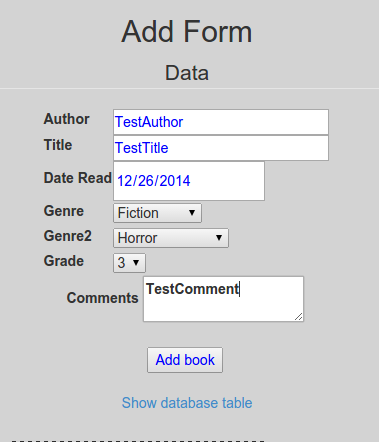
\includegraphics[width=70mm, height=80mm]{del2_addbook.png}
		\caption{Formulär med korrekt ifyllda fält}
		\end{figure}
		
		Resultat:
		\begin{figure}[ht!]
		\centering
		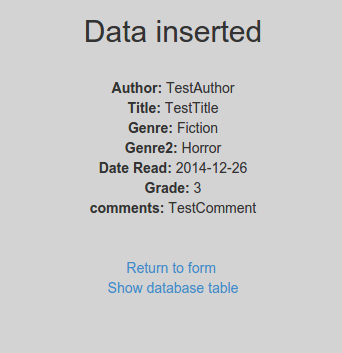
\includegraphics[width=70mm, height=80mm]{del2_addbook_res.png}
		\caption{Resultat}
		\end{figure}
		
		
		\newpage
		\textbf{Test 2: Felaktig Author} \\
		Jag skriver in i \emph{Author} fältet: \textbf{fel1}, \emph{Author} får ej innehålla siffror.
		
		\begin{figure}[ht!]
		\centering
		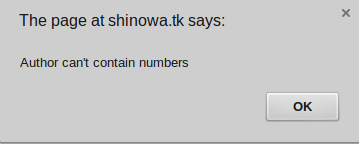
\includegraphics{del2_felauthor.png}
		\caption{Resultat}
		\end{figure}
		
		Kommentar: När jag trycker på Add book så visas denna popup.
		
		\textbf{Title} \\
		Titel får innehålla alla tecken, inget att testa.
		
		\textbf{Felaktigt Datum} \\
		Är av typen date i formuläret så det är svårt att göra fel i detta fält. Man kan däremot mata in konstiga år tex: 123123, lite långt i framtiden kanske.
		
		\textbf{Genre} \\
		Går ej att göra fel på.
		
		\textbf{Genre2} \\
		Genre2's lista uppdateras beroende på vilken värde som \emph{Genre} har, detta har jag testat manuellt och det verkar fungera felfritt.
		
		\textbf{Grade} \\
		Går ej att göra fel på.
		
		\textbf{Comments} \\
		Får vara tom och innehålla alla sorters tecken, så inget att testa här.
		
		\newpage
		\Subsubsection{Ta bort bok}
		\textbf{Test 1: ta bort en titel som finns}\\
		Jag skriver in en titel som jag vet finns i databasen vid testets tidpunkt.
		\begin{figure}[ht!]
		\centering
		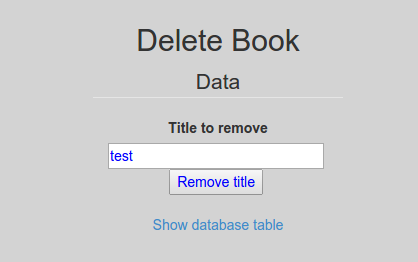
\includegraphics[width=70mm, height=80mm]{del2_del.png}
		\caption{Titel att ta bort}
		\end{figure}
		
		Resultat:
		\begin{figure}[ht!]
		\centering
		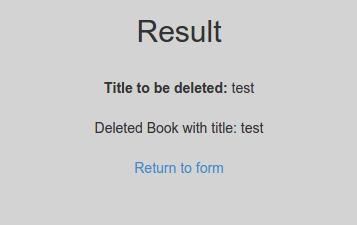
\includegraphics[width=70mm, height=80mm]{del2_del_res.png}
		\caption{Resultat}
		\end{figure}
		
		\newpage
		\textbf{Test 2: Ta bort titel som inte finns} \\
		Jag försöker ta bort titeln: finnsinte.
		
		\begin{figure}[ht!]
		\centering
		
\includegraphics[width=70mm, height=80mm]{del2_delfail.png}
		\caption{Resultat}
		\end{figure}
		
		\Subsubsection{Ändra bokdata}
		Innehåller samma delar som används för att lägga till en bok, så tester på denna del kommer att ge samma resultat som \emph{Add book} formuläret för att de använder samma funktion för att valideras. 
		
		
	\Section{Diskussion}
 Jag har i mina lösningar valt att prova två stycken sätt att validera datat som skrivs in i formulären, i del 1 så använder jag php för detta och det fungerar bra, det negativa med detta
 är att användaren måste gå tillbaka och skriva om det som är fel.
 I del två så använder jag javascript och när användaren ska submitta så kontrolleras alla fält och en popup visas om något är fel utan att webbläsaren byter sida.
 Jag personligen tycker att del 2's lösning är bättre för det går snabbare att ändra formuläret så det blir korrekt och det behöver inte läggas ner tid på att visa en ny sida i webbläsaren och användaren behöver inte klicka \emph{Back}.

 Jag har inte hållit på med php förrut och det jag tycker var svårt med php är det att man bakar in html kod i php koden, det kändes svårt att få koden lättläslig när man blandar html och php, 
 men detta kan vara en vanesak samt att det kan finnas bättre sätt att skriva vissa delar på än vad jag lyckats åstadkomma.
 
 När det gäller formulären så hjälper de typer man kan sätta de olika inputfälten till väldigt mycket, email, date number är mycket smidiga eftersom att dom själva ser till så att användaren bara kan skriva in
 något i fältet som är korrekt.
 
 Jag har användt PDO med parametriserade \emph{Queries} för mysql delen för att försöka att göra det \emph{Sql-Injection} säkert men jag har ingen tidigare erfarenhet av databaser eller \emph{Sql-Injection} så det är nog inte supersäkert.
 Får gärna försöka att titta om det går att förstöra databasen då det troligen finns mera erfarenhet av sånt för dig som rättar.
 
\end{document}